\section{Local Oscillator}

\begin{frame}{Local Oscillator}

    Normally, the local oscillator in a CSAC is a quartz crystal oscillator (XO).

    There exist many versions of the XO, differentiated based on the environmental correction type applied to enhance stability:

    \begin{itemize}
        \item \textbf{TCXO}: Temperature Compensated Crystal Oscillator
        \item \textbf{MCXO}: Microcomputer Compensated Crystal Oscillator
        \item \textbf{OCXO}: Oven Controlled Crystal Oscillator
    \end{itemize}

\end{frame}



\begin{frame}{Quartz Crystal Oscillator}

    \textbf{At short time scales, the quartz crystal oscillator is the main source of instability} in a CSAC due to its phase noise.

    \begin{columns}[c, onlytextwidth]

        \begin{column}{0.6\textwidth}

            Here are some other problematic areas:

            \begin{itemize}
                \item High temperature sensitivity
                \item Power consumption (due to thermal control to enhance stability)
                \item Aging and frequency drift
            \end{itemize}

        \end{column}

        \begin{column}{0.4\textwidth}

            \begin{figure}
                \centering
                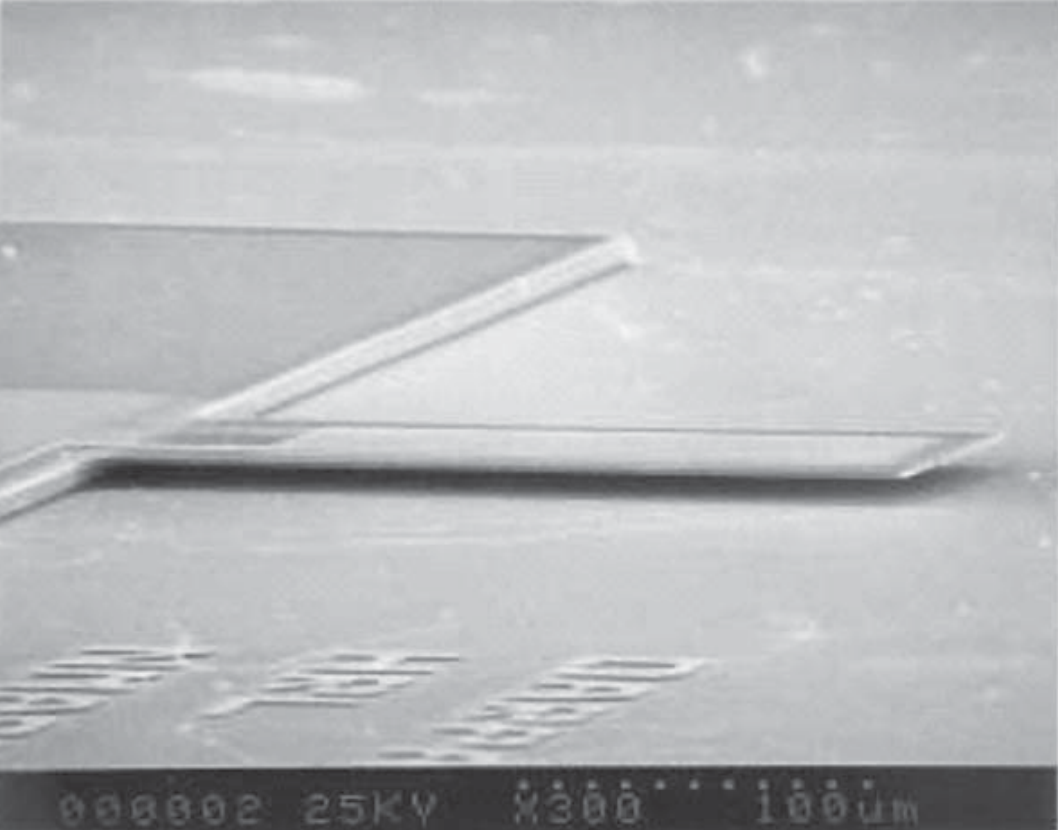
\includegraphics[width=0.9\textwidth]{img/thin-local-oscillator.png}
                \caption{Resonator with 2-mm quartz thickness\footnotemark[1].}
            \end{figure}

        \end{column}

    \end{columns}

    In the end, the choice of a local oscillator is a trade-off between stability and power consumption.

    \footnotetext[1]{Photograph taken using Scanning Electron Microscope (SEM) technique.}

\end{frame}